\title{Parametric RSA applied to Mixed-Gambles Task}
\author{Charles Zheng, Sanmi Koyejo and Russ Poldrack}
\date{\today}

\documentclass[12pt]{article} 

% packages with special commands
\usepackage{amssymb, amsmath}
\usepackage{epsfig}
\usepackage{array}
\usepackage{ifthen}
\usepackage{color}
\usepackage{fancyhdr}
\usepackage{graphicx}
\usepackage{mathtools}
\usepackage{csquotes}
\definecolor{grey}{rgb}{0.5,0.5,0.5}

\begin{document}
\maketitle

\newcommand{\tr}{\text{tr}}
\newcommand{\E}{\textbf{E}}
\newcommand{\diag}{\text{diag}}
\newcommand{\argmax}{\text{argmax}}
\newcommand{\Cov}{\text{Cov}}
\newcommand{\Var}{\text{Var}}
\newcommand{\argmin}{\text{argmin}}
\newcommand{\Vol}{\text{Vol}}
\newcommand{\comm}[1]{}

\newcommand{\bx}{\boldsymbol{x}}
\newcommand{\by}{\boldsymbol{y}}
\newcommand{\bX}{\boldsymbol{X}}
\newcommand{\bY}{\boldsymbol{Y}}


\section{Introduction}

Representational similarity analysis (Kriegeskorte et al.) is a distance-based approach
for comparing how different subjects or different parts of the brain
differ in perceiving a given fMRI task.
Let $i = 1,\hdots, k$ index a collection of tasks,
and let $r = 1,\hdots, n$ index a set of \emph{representators} to be compared.
A representator could be:
\begin{itemize}
\item The whole brain of a subject.
\item A region of a subject's brain.
\item A model-based prediction of the activity of a brain or region of interest.
\item The subject's behaviorial response to the task (e.g. responses to survey questions)
\item A manual labelling of the task into categories.
\end{itemize}

Each representor produces a representation of each stimulus, denoted $y^{(i, r)}$.
The representation could be categorical, scalar-valued or multidimensional,
or even non-numerical, e.g. text descriptions.
Furthermore, the different representors could produce representations of different types.
What is essential to the approach is a way to compute distances between representations coming
from the same representor, i.e. a $k \times k$ distance matrix
$d^{(r)}(i, j)$ of pairwise distances between stimuli, for $r = 1,\hdots, n$.
Representational similarity analysis works by comparing these $n$ distance matrices
in order to draw conclusions about the nature of the representors.

Suppose that the representators all produce real, vector-valued representations, of possibly differing dimensionality $v_r$.  Furthermore, suppose we choose the squared Euclidean distance
\[
d^{(r)}(i, j) = \frac{1}{v_r} ||y_{(r, i)} - y_{(r, j)}||^2.
\]
Here we divide by $v_r$ so that in the commonly encountered case where the representation is obtained by
sampling from a continuous function, the resulting distance is robust to fineness of discretization.

In many experimental designs, we have a parameterization of the stimuli, given by a vector $x_i$.

\section{Data}

We used the mixed-gambles data from Tom et al. 2007.
The data consisted of 3 runs for each of 16 subjects.
In each run, 16 different gambling tasks were presented.
These tasks varied in the gain amount and loss amount.

Clusters were obtained using a parametric map from {\tt http://neurovault.org/images/10680/},
then applying thresholding using FSL.
A size threshold was applied, yielding 28 regions of interest.

\begin{figure}[h]
\centering
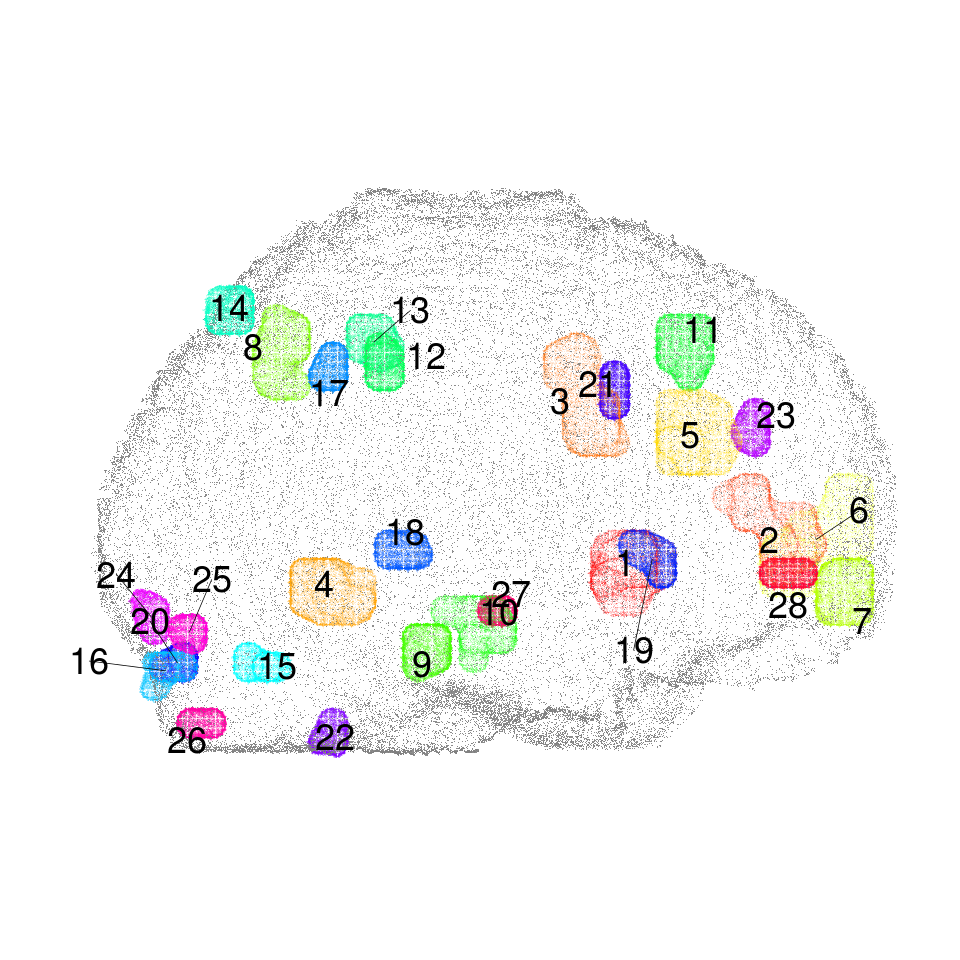
\includegraphics[scale = 0.1]{../a7plots/all_rois_view1.png}
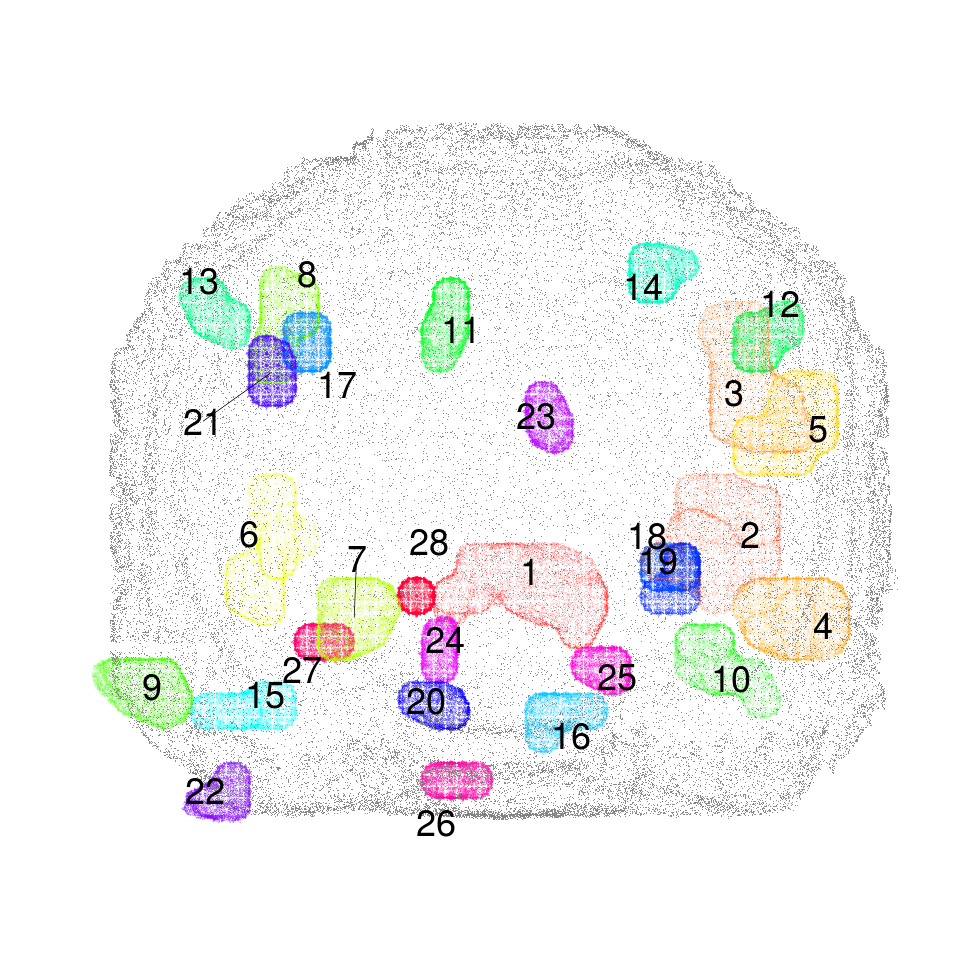
\includegraphics[scale = 0.1]{../a7plots/all_rois_view2.png}
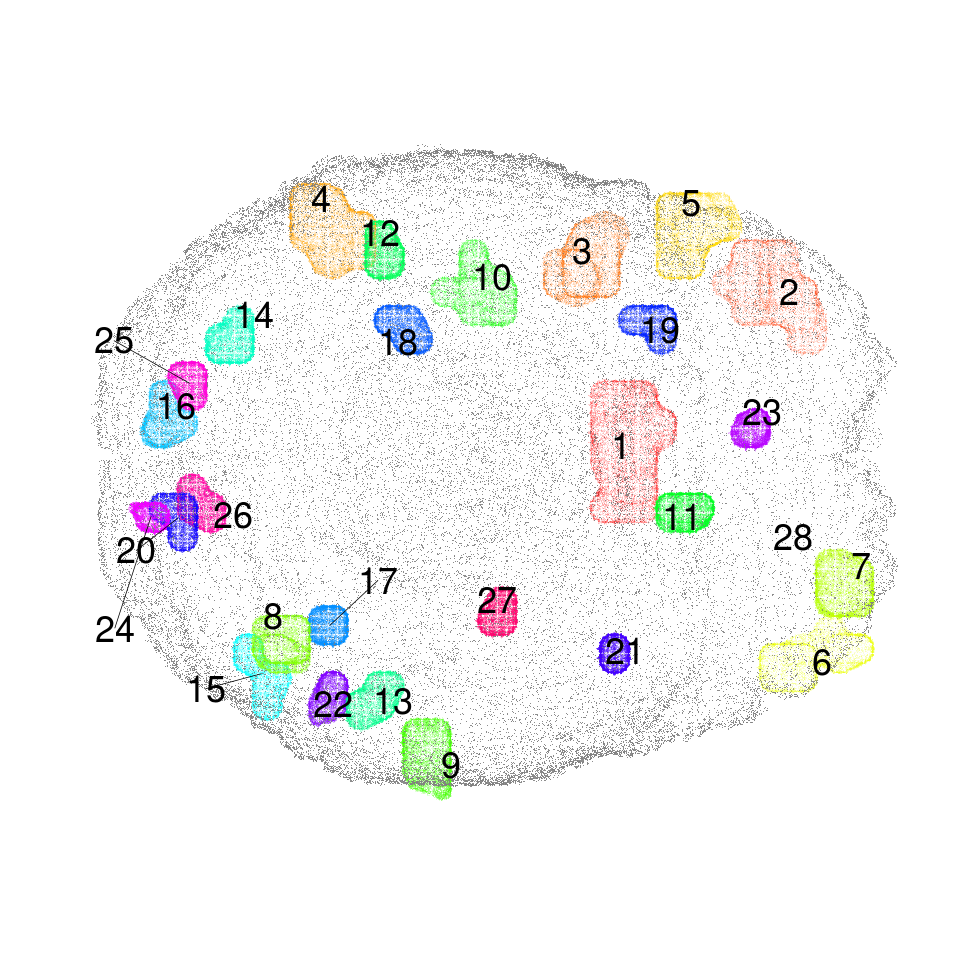
\includegraphics[scale = 0.1]{../a7plots/all_rois_view3.png}
\caption{Regions of interest.}
\end{figure}

The scans were registered to a common template, then a standard linear model-based approach
was used to extract an activity level per voxel per event per run.
We extracted the regions of interest from the data.  For a given region of interest, the data takes the form:

\begin{tabular}{|c|c|c|c||c|c|c|c|}
\hline
subject & run & gain & loss & voxel 1 & voxel 2 & ... & voxel $N$ \\
\hline
 1 & 1 & 13 &  6.5 & -222.8994 &  -373.85025 & ... & 12.038\\
... & ... & ... & ... & ... & ... & ... & ...\\
16 & 3 & 37 & 18.5 & -136.89 & -73.49 & ... & 75.068146 \\
\hline
\end{tabular}

where $N$ is the number of voxels in the ROI.

\section{Methods}

We model the data using the following linear model.
Let $s = 1,\hdots, 16$ index the subjects, and $e = 1,\hdots, 48$ index the events from all runs combined.
Let $r = 1,\hdots, 28$ index the regions of interest, and $m = 1,\hdots, v_r$ the voxels in the ROI.
Then the model for the activity of the $m$th voxel in the $r$th roi is
\[
y_{s, e, r, m} = \langle \vec{x}_{e}, \beta_{s, r, m} \rangle + \mu_{s, r, m} + \epsilon_{s, e, r, m}
\] 
where $y_{s, e, r, m}$ is the activity of the $m$th voxel for the $s$th subject in the $e$th event (a scalar quantity),
$\vec{x}_e$ is the 2x1 vector of parameters (gain and loss) for the $e$th event ,
and $\beta_{s, r, m}$ is a vector of coefficients specific to the subject and to the voxel.
The coefficient vector $\beta_{s, r, m}$ is viewed as a \emph{random effect} such to variation between subjects.
$\mu_{s, r, m}$ is a subject-specific mean term for the voxel.
Meanwhile, assume that the noise term $\epsilon_{s, e, r, m}$ is normal $N(0, \sigma^2_{s, r, m})$
with zero mean, and covariance specific to the subject and voxel.
Assume that the noise terms for are correlated \emph{within an event} but are independent \emph{across events}.  This assumption may not be realistic, since there is usually some autocorrelation across events.
\[
\text{ if }e \neq e' \text{ or }s \neq s', \text{ then }\Cov(e_{s, e, r, m}, e_{s', e', r, m}) = 0 .
\]
\[
\Cov(e_{s, e, r, m}, e_{s, e, r', m'}) = \sigma_{r,m,r',m'}.
\]
Write $\Sigma_{r}$ for the $n_v \times n_v$ covariance matrix for voxels within a region of interest.

The parametric RSA approach is to define for each subject and ROI the feature-distance matrix $M^{(s, r)}$ with entries
\[
M^{(s, r)}_{ij} = \frac{1}{v_r}\langle \beta_{s, r, i}, \beta_{s, r, j }\rangle.
\]
The randomness of $\beta_{s, r, m}$ induces a random distribution for $M^{(s, r)}$ for a given randomly sampled subject. Let $F^{(r)}$ denote the distribution of the $2 \times 2$ matrix $M^{(s, r)}$.

We are interested in comparing feature-distance matrices across regions of interest.
Suppose we wish to compare region $r$ with region $r'$.  The null hypothesis is that
\[
H_0: \E[M^{(s, r)}] = \E[M^{(s, r')}]
\]
where the expectation is taken across the distribution of subjects.


\end{document}



